\documentclass[11pt]{article}
\usepackage[utf8]{inputenc}
\usepackage[T1]{fontenc}
\usepackage[letterpaper,margin=0.75in,includehead=false]{geometry}
\usepackage{graphicx}
\usepackage{fancyhdr}
\usepackage{parskip}
\usepackage{url}
\usepackage{float}
\usepackage{caption}
\usepackage{tabularx}
\usepackage{booktabs}
\usepackage{longtable}
\usepackage{array}
\usepackage{enumitem}
\usepackage{xcolor}
\usepackage{xspace}
\usepackage{tikz}
\usetikzlibrary{arrows.meta, positioning, fit, calc}
\captionsetup{font=it}
\captionsetup{justification=centering}
\setlist{itemsep=0.1em, topsep=0.2em}
\emergencystretch=2em
\setlength{\headheight}{42pt}
\pagestyle{fancy}
\fancyhf{}
\fancyhead[R]{
\includegraphics[height=0.45in]{../artifacts/logo.png}}
\fancyfoot[C]{\thepage}
\renewcommand{\headrulewidth}{0pt}


\tikzset{
  box/.style={draw, rounded corners=2pt, align=center, font=\footnotesize, inner sep=4pt, minimum height=0.8cm, fill=gray!8},
  grp/.style={draw, dashed, rounded corners=3pt, inner sep=6pt},
  arr/.style={-{Stealth[length=2mm]}, thick},
  lbl/.style={font=\scriptsize, fill=white, inner sep=1.5pt, align=center}
}

\begin{document}
\begin{titlepage}
  \centering
  \vspace*{1in}
  {\fontsize{25pt}{30pt}\selectfont\textbf{R3: Preliminary Report}\par}
  \vspace{0.5in}
  {\LARGE\textbf{CEN4908 CpE Design 2}\par}
  \vspace{0.35em}
  {\Large Hardened RISC-V Exam Computer\par}
  \vspace{0.3em}
  {\Large October 28, 2026\par}
  \vspace{0.6in}
  {\Large Cannon Spencer \quad George Rushevich \quad Justin Reyes \quad Gabriel Velazquez\par}
  \vspace{1in}
  
\includegraphics[height=1.65in]{../artifacts/uf-logo.png}\hspace{1.25in}%
  
\includegraphics[height=1.65in]{../artifacts/big-logo.png}\par
\end{titlepage}
\newpage
\setcounter{page}{1}

%=============================================================================

%=============================================================================
\section*{Abstract}
%=============================================================================

AI tools have made it easier than ever to cheat on exams, and the most common countermeasure, proctoring software such as Honorlock, works by monitoring students on their own laptops. We take a different approach: a small exam computer that the university owns and hands out at test time. Our device is an Orange Pi RV, a RISC-V single-board computer, running the manufacturer's Debian image with Safe Exam Browser (SEB)~\cite{safeexambrowser} locked full-screen inside the cage kiosk compositor~\cite{cage_kiosk}, where students take their exam in Canvas. Because SEB has no official Linux or RISC-V release and Chromium is not packaged for riscv64, we run a community Linux port of SEB~\cite{seblinux} built on WebKitGTK. Instructors start and stop exams across every board from a web console. The boards reach our server over HTTPS through a Cloudflare tunnel, so they work on campus Wi-Fi without exposing any ports. Starting an exam sends each board that exam's \texttt{.seb} configuration, and the server releases the Canvas quiz access code only after verifying SEB's Config Key, so the quiz cannot be opened from an ordinary browser. Flashing a board, installing our software, and launching SEB from the server all work today, and a single command has started SEB on two boards at once. By rebuilding WebKitGTK for OpenGL~ES, we also moved SEB's rendering onto the board's PowerVR GPU. Canvas remains too slow for a real exam, however: its JavaScript saturates one 1.5\,GHz core, and one post-login page took more than two minutes to load. For the rest of the term, we plan to reduce what Canvas loads, boot the board directly into the kiosk, and finish the instructor console and related tools.

%=============================================================================
\section{Introduction}
%=============================================================================
A growing share of exams are now taken on a computer, in the classroom and remotely, and generative AI has made those exams much harder to trust. With an AI tool open in another window or on a second device, a student can get help on nearly any kind of question, from short answers to essays to code. Instructors have largely been left with two options: return to paper, or require proctoring software such as Honorlock or Respondus. Proctoring software runs on the student's own laptop and monitors the student, their screen, and their surroundings for the length of the exam, asking students to give up a considerable amount of privacy on a machine they personally own.

Our project takes a different route. Rather than trying to lock down whatever laptop a student brings, the university provides a small exam computer that it owns and controls. The device boots directly into Safe Exam Browser (SEB)~\cite{safeexambrowser} and opens the exam in Canvas. There is no desktop to fall back to, nothing for the student to install, and nothing ever placed on the student's personal machine. Any course that already delivers exams through Canvas could adopt it. Our work covers both the device itself and the tools an instructor needs to run a full room of them.

This is a faculty project under Dr.~Blanchard, with the goal of using these boards for in-class exams in UF courses.

\textbf{How the plan has changed.} Our design draft called for a custom, hardened Linux image on the Banana Pi BPI-F3, with secure boot and RISC-V memory protection. We have since moved to the Orange Pi RV, and we now build its image with the manufacturer's own Debian build system (Debian sid with GNOME), since the GNOME desktop build is the configuration that installs this chip's GPU libraries. Lockdown now comes from running SEB as the only application inside a cage kiosk. OS-level hardening (dm-verity and signed boot) is documented but is not part of the current image.

%=============================================================================
\section{Background}
%=============================================================================

\textbf{Prior art.} Honorlock and Respondus run on the student's computer. SEB~\cite{safeexambrowser} (ETH Z\"urich) is a well-known lockdown browser, officially only for Windows, macOS and iOS; its documentation~\cite{seb_concept} explains how a config file, URL filters and keys tie it to one exam. \texttt{seb-linux}~\cite{seblinux} ports it to Linux and falls back to WebKitGTK when Qt6 WebEngine is missing, which is what makes riscv64 possible. Cage~\cite{cage_kiosk} is a Wayland compositor that shows one app full-screen.

\textbf{SEB Config Key.} SEB sends \texttt{X-SafeExamBrowser-ConfigKeyHash} with each request: the SHA-256 of the URL plus the exam's Config Key. A server that knows the key can tell the request came from SEB running that exact config. Our \texttt{proto} crate computes Config Keys and is tested against files made by real SEB.

\textbf{The board.} We first looked at the Banana Pi BPI-F3 (SpacemiT K1, 8 cores)~\cite{spacemit_k1} and the RISC-V privileged spec's PMP~\cite{riscv_priv} for hardening. We are now on the Orange Pi RV: a StarFive JH7110 with 4 cores at 1.5\,GHz, 8\,GB of RAM and a PowerVR BXE-4-32 GPU whose vendor driver only does OpenGL~ES. The open-source Mesa PowerVR driver lists this GPU as unsupported.

%=============================================================================
\section{Design}
%=============================================================================

\subsection{Overview}
There are three parts (Figure~\ref{fig:arch}): exam boards, a control server, and the instructor console the server hosts. Boards always connect to the server, never the reverse, so they have no open ports and work on campus networks that block incoming connections.

\begin{figure}[H]
\centering
\begin{tikzpicture}[x=1cm,y=1cm]
  \node[box, text width=3.0cm] (inst) at (0,0) {Instructor browser\\(console, login)};
  \node[box, text width=4.6cm] (cf) at (5.6,0) {Cloudflare tunnel (HTTPS)\\{\scriptsize\texttt{riscv-exam-computer.download}}};
  \node[box, text width=3.4cm] (srv) at (12.0,0) {Exam server (Rust, Axum)\\fleet, exams, gate,\\JSON persistence};
  \node[box, text width=3.0cm] (seb) at (0,-3.6) {SEB (WebKitGTK)\\in cage kiosk};
  \node[box, text width=3.0cm] (agent) at (5.6,-3.6) {\texttt{seb-agent}\\systemd user unit};
  \node[box, text width=3.4cm] (canvas) at (12.0,-3.6) {Canvas, UF login, Duo};
  \node[grp, fit=(agent)(seb), label={[font=\scriptsize]above:Orange Pi RV board (one of many)}] (board) {};
  \draw[arr,<->] (inst) -- node[lbl,above]{HTTPS} (cf);
  \draw[arr,<->] (cf) -- node[lbl,above]{HTTP :8000} (srv);
  \draw[arr,<->] ([xshift=6mm]agent.north) -- node[lbl,right]{heartbeat / 5\,s;\\job + \texttt{.seb} in reply} ([xshift=6mm]cf.south);
  \draw[arr] (agent) -- node[lbl,above]{\texttt{sudo -n}} (seb);
  \draw[arr] (seb.north) -- node[lbl,left,pos=0.72]{gate: Config Key hash} ([xshift=-6mm]cf.south);
  \draw[arr,<->] (seb.south) -- ++(0,-0.9) -| node[lbl,below,pos=0.25]{HTTPS, allowlisted domains only} (canvas.south);
\end{tikzpicture}
\caption{System architecture and communication paths.}
\label{fig:arch}
\end{figure}

\subsection{Exam board}
CI in \texttt{reptilian-riscv} uses Orange Pi's build system to make U-Boot and a Debian sid GNOME image; we use the desktop build because it is the one that installs the GPU libraries. \texttt{flash-os.sh} writes it to an SD card. \texttt{install-seb.sh} copies a prebuilt riscv64 SEB from a GitHub release (building on every board kept failing). \texttt{install-gpu.sh} adds our GPU stack: WebKitGTK rebuilt for GLES, patched wlroots and cage, and the kiosk launchers. \texttt{install-software.sh} adds \texttt{seb-agent}, its start and stop scripts, and a sudoers rule for only those two scripts (Figure~\ref{fig:stack}).

\begin{figure}[H]
\centering
\begin{tikzpicture}[x=1cm,y=1cm, every node/.style={box, minimum width=11cm}]
  \node at (0,4.0) {Canvas exam page, UF login, Duo (remote web content)};
  \node at (0,3.0) {Safe Exam Browser (\texttt{seb-linux}: Qt6 shell, WebKitGTK engine rebuilt for GLES)};
  \node at (0,2.0) {cage 0.1.4 + wlroots 0.15.1 (patched), on tty7 at 1280$\times$720 \; [X + openbox fallback]};
  \node at (0,1.0) {Vendor Debian sid (GNOME build), kernel 5.15 \texttt{starfive2}, IMG GPU userspace; \texttt{seb-agent}};
  \node at (0,0.0) {Orange Pi RV: JH7110 (4 cores, 1.5\,GHz), 8\,GB RAM, PowerVR BXE-4-32, SD card, Wi-Fi, HDMI, USB};
\end{tikzpicture}
\caption{Board software and hardware layers.}
\label{fig:stack}
\end{figure}

\textbf{Kiosk.} SEB runs inside cage on tty7 as a systemd unit. In lockdown mode SEB normally takes over its own console and draws straight to the framebuffer, which leaves WebKit no compositor and breaks the GPU path; cage fixes that. We patched wlroots to accept the GLES 3 driver, patched cage to force 1280$\times$720, and added a flag so SEB skips its console switch inside cage. Without the GPU stack, \texttt{start-seb.sh} falls back to X and openbox on the CPU.

\textbf{Agent.} Every 5\,s \texttt{seb-agent} sends a JSON heartbeat (host name, \texttt{idle}/\texttt{running}, protocol 3, versions, current exam, last job result), with a bearer token if one is set. A \texttt{start} reply carries the exam's \texttt{.seb}; the agent writes it to \texttt{\textasciitilde/exam.seb} through a temp file and rename, then runs the start script.

\textbf{Mount.} A 3D-printed bracket (\texttt{docs/cad}) puts the board on a monitor's VESA holes, so a station is just a monitor, keyboard, mouse and power.

\subsection{Control server and console}
The server is Rust with Axum, and the console is a server-rendered Leptos app. GitHub Actions builds the container image, and \texttt{deploy-server.sh} runs it in Docker behind the tunnel. It stores boards, jobs (each with an ID, timeout and per-board result), exams and an activity log in a JSON file, written to a temp file, synced and renamed so it can't be half-written. Instructors pick boards and an exam and start or stop them, and the console shows which boards were skipped and why. Status is always an icon, a word and a color (\texttt{exam-env/DESIGN.md}). Login needs a password, attempts are rate-limited, and cross-origin changes are rejected. \texttt{sim-agent} fakes any number of boards, including failing ones.

\subsection{Exam delivery and the SEB gate}
An exam is a start URL, allowed domains, whether students may quit, and the Canvas quiz access code. The server builds a \texttt{.seb} from that and computes its Config Key; URL rules are anchored regexes so one site's rule can't match another site. The exam starts at our \texttt{/gate/\{id\}} page. The server recomputes the hash for that URL and compares it with SEB's header: on a match it shows the access code, otherwise it refuses and logs it. SEB versions that only expose the key to JavaScript get a small page that posts it back for the same check. A normal browser never sees the code.

\subsection{Communication}
Boards use Wi-Fi (registered on campus \texttt{ufdevice}) or Ethernet. All traffic is JSON over HTTPS to Cloudflare, which forwards HTTP to the server on port 8000. We SSH to boards through Tailscale on campus, since eduroam blocks laptop-to-board SSH, and use a 115200-baud UART console for first boot. Display is HDMI; input is USB.

\subsection{Risks and mitigations}
\begin{table}[H]
\centering
\footnotesize
\begin{tabularx}{\textwidth}{@{}p{0.28\textwidth}X@{}}
\toprule
\textbf{Risk} & \textbf{Mitigation} \\
\midrule
Canvas too slow & GPU compositing done; next, quiz-URL start, domain allowlist, kiosk-only boot; faster hardware not yet researched. \\
Quiz opened outside SEB & Gate gives the access code only to SEB with that exam's config (done). \\
Kiosk escape & SEB is the only app in cage; exit-path test LD-01 still to run. \\
Board software changed & dm-verity written up, not in image; signed boot deferred. \\
Physical attacks (GPIO, keyloggers) & Raised in the design draft; not addressed this term. \\
Unauthorized start/stop & Password login, agent token, origin checks (done). \\
Board fails mid-exam & Swap boards; agent restarts itself, jobs time out, server state is saved. \\
Overheating, display glitches & Heatsink or fan, then retest (9/30 log). \\
\bottomrule
\end{tabularx}
\caption{Risks and mitigations.}
\end{table}

%=============================================================================
\section{Tools, Design Constraints, and Engineering Standards}
%=============================================================================

\textbf{Tools.} Git, GitHub (releases and Actions) and Jira; Rust with \texttt{cargo-zigbuild}, Axum, Leptos, Docker, \texttt{cloudflared} and Tailscale; the Orange Pi build system, Qt6, WebKitGTK, wlroots and cage; gdb, \texttt{screen}/PuTTY for UART, balenaEtcher and \texttt{dd}; CAD for the mount; \LaTeX.

\textbf{Standards.} RISC-V privileged spec~\cite{riscv_priv}; HTTPS/TLS, HTTP, JSON and cookies; Wi-Fi; SHA-256 and the SEB config and key formats~\cite{seb_concept}; Wayland, X11 and OpenGL~ES; GPT and ext4; HDMI, USB, UART and VESA mounting; the ARIA/ADA goals from the design draft.

\textbf{Constraints.}
\begin{itemize}
  \item No Qt6 WebEngine on riscv64, so SEB uses WebKitGTK, whose Debian build wants desktop OpenGL that this GPU lacks.
  \item The GPU stack needs kernel 5.15 and a frozen 2022-12-25 Debian snapshot (no \texttt{apt upgrade}); the GLES WebKit rebuild took about 11.5 hours on the board.
  \item The cores already run at their 1.5\,GHz maximum.
  \item Canvas is the university's choice; we can only reduce what it loads.
  \item Campus networks block incoming connections and laptop-to-board SSH.
  \item Staying on the vendor image keeps the GPU but makes a hardened custom OS harder this term.
  \item One semester, four people.
\end{itemize}

%=============================================================================
\section{Needs and Impact Analysis}
%=============================================================================

The need is the same as in the design draft: exams instructors can trust, without surveilling students' own computers.

\textbf{Social and cultural.} If the exam can't be bypassed, students have a reason to learn the material, everyone tests under the same conditions, and a UF degree keeps its meaning.

\textbf{Economic.} Honorlock and Respondus charge per student and per exam, which can reach six-figure annual fees; a university-owned fleet replaces that with an upfront hardware cost, and maintaining it could be a student job.

\textbf{Environmental and global.} RISC-V is an open instruction set, the boards draw under 15\,W, far less than a lab of laptops, and the mounts can be printed in recyclable PLA or PETG.

\textbf{Ethical and professional.} Nothing is installed on a student's computer. Our logs and this report state plainly that Canvas is not yet fast enough on this board, and setting expectations with stakeholders is an open item. The console treats board-supplied text as untrusted, and secrets stay out of the repository. The design draft commits to screen-reader (ARIA) and keyboard-only support.

\textbf{Limitations.} Canvas isn't exam-usable yet (Section~\ref{sec:results}). The image is a stock desktop with a writable root, so physical access means it can be changed. The server runs on one laptop, and only one laptop can run the tunnel. The GPU stack depends on a vendor driver and an old snapshot. The current SEB release is missing the WebKitGTK extension that does URL filtering and sends the SEB key headers; \texttt{install-seb.sh} calls this temporary, so the gate and URL filter still need to be confirmed on a board.

\textbf{Future work.} The design draft's stretch goals still apply: central config distribution, per-device keys, and OS hardening (dm-verity, kernel lockdown, secure boot). A faster board is the only direct fix for the CPU limit, and most of the cage and SEB work should carry over. WebKitGTK 2.46+ renders with Skia, which Igalia reports often suits embedded chips better (from our 9/24 research notes); Debian trixie ships 2.52 for riscv64 but needs glibc 2.38+.

%=============================================================================
\section{Results}
\label{sec:results}
%=============================================================================

Full procedures and pass criteria are in our T1 and T2 test plans (\texttt{docs/latex/}); dated lab notes are in \texttt{docs/log/}.

\subsection{Alpha (T1, September 2026)}
\begin{table}[H]
\centering
\footnotesize
\begin{tabularx}{\textwidth}{@{}p{0.08\textwidth}p{0.20\textwidth}X@{}}
\toprule
\textbf{ID} & \textbf{Test} & \textbf{Result} \\
\midrule
HW-01 & Flash and boot & Pass. The image boots to a login over UART at 115200 baud. \\
HW-02 & SSH & Pass on a lab network. On campus we needed \texttt{ufdevice} and Tailscale. \\
HW-03 & Outbound network & Pass. \texttt{ping -c 4} showed 0\% loss over Wi-Fi. \\
SW-01 & SEB binary on board & Pass, but we changed the approach: building SEB on each board kept failing, so we now build it once and install it from a release. \\
INT-01 & SEB launches & Pass. Canvas clicks took 10\,s or more, and the page drew in tiles. \\
INT-02 & Lockdown smoke test & Not run. We moved it to beta as LD-01. \\
SW-02 & Agent heartbeat & Pass, both to a LAN listener and through the tunnel. \\
\bottomrule
\end{tabularx}
\caption{Alpha results (also summarized in T2).}
\end{table}

\subsection{Beta (T2, October 2026)}
\textbf{Two-board demo (DEMO-01).} On October~2, one \texttt{POST /start} queued \texttt{orangepirv1} and \texttt{orangepirv2}, SEB came up on both within 90\,s, and \texttt{/stop} returned both to the console. That met the beta goal but was well over our proposed 10\,s start time (R-T3).

\textbf{Outside users.} Two non-team students each used a board for about 5 minutes. Both logged in and used Canvas on their own, and both commented on how slow it was. On a repeat, a failed UF login sent one to \texttt{ufl.edu}, and SEB's navigation lockdown left no way back (BUG-03).

\textbf{GPU.} We checked which libraries WebKit's web process had loaded (\texttt{/proc/<pid>/maps}); \texttt{pvr\_dri.so} and the IMG GLES libraries only load when a GPU context is created. Stock WebKit failed with ``Could not create EGL context.'' After the GLES rebuild they loaded for MiniBrowser on the desktop, as root and in cage, and for SEB in cage. Without \texttt{GDK\_GL=gles} or \texttt{MESA\_LOADER\_DRIVER\_OVERRIDE=pvr} they were missing, so the result depends on the setup and isn't a coincidence. DRM state confirmed 1280$\times$720 at 60\,Hz. Pass.

\textbf{Where the time goes.} With Canvas open, \texttt{top} showed SEB's WebKit process at 100\% of one core while the system sat near 44\%, with the governor already at 1.5\,GHz. Perf counters aren't available in this kernel, so we paused the main thread in gdb 33 times: about 42\% JavaScript, 39\% unlabeled SEB/Qt code, 12\% layout and paint, 6\% idle. One timed run from the post-Duo page to the course page took over 2 minutes. We hoped the GPU would make Canvas usable; it didn't. With only 33 samples and no pre-GPU baseline, these numbers are rough.

\textbf{Long runs and heat.} Two runs of about 12 hours each had no crashes. The board hit about 75\,\textdegree C with no heatsink in a 73\,\textdegree F room, too hot to touch, and the display flashed or tore a few times until an HDMI replug or cooldown. Temperature wasn't logged continuously, so this still needs a proper thermal test.

\textbf{Automated tests.} \path{exam-env/proto}, \path{exam-env/server/src} and \path{exam-env/server/tests/http.rs} hold unit and HTTP tests for Config Keys (against SEB-made files), job lifecycle and timeouts, bad input, agent tokens, login rate limits, and the gate accepting the right key and rejecting a wrong one.

\textbf{Still to run.} No results are recorded yet for LD-01 (exit paths), SES-03 (repeated start/stop), AGT-03 to AGT-05 (outage, crash, boot recovery) or PERF-01 to PERF-04. These are planned before the final report.

\subsection{What we changed because of testing}
\begin{itemize}
  \item On-board SEB builds kept failing, so we ship one release binary.
  \item Our Oracle VM ran out of memory and campus blocks incoming connections, so the server moved to a laptop behind a Cloudflare tunnel with outgoing-only boards.
  \item Lab launches used a hand-made start file; the server now generates and sends each exam's \texttt{.seb}.
  \item Beta had no auth, an in-memory board list and broadcast-only start/stop (LIM-01 to LIM-03); we added login, rate limits, origin checks, agent tokens, saved state, job IDs and timeouts, and per-board selection.
  \item SEB without a compositor couldn't use the GPU, so we moved it into cage.
  \item Profiling showed JavaScript, not graphics, is the problem, which led to the plans above: quiz-URL start, an allowlist, kiosk-only boot, and maybe different hardware.
\end{itemize}

%=============================================================================
\section{Status}
%=============================================================================
\begin{longtable}{@{}p{0.15\textwidth}p{0.16\textwidth}p{0.62\textwidth}@{}}
\toprule
\textbf{When} & \textbf{Status} & \textbf{Item} \\
\midrule
\endhead
Sep 4--10 & Done & Debian boots on the board; \texttt{seb-linux} WebKitGTK fixes; SEB shows Canvas. \\
Sep 7--16 & Done & CI image and \texttt{flash-os.sh}; agent cross-compile and install; first heartbeats. \\
Sep 23--25 & Done & Server behind Cloudflare tunnel; campus SSH; SEB release binary and \texttt{install-seb.sh}. \\
Sep 30--Oct 2 & Done & Start/stop jobs; kiosk scripts; two-board demo; beta build. \\
Sep 24--Oct 22 & Done & GPU stack (GLES WebKitGTK, patched wlroots and cage) and \texttt{install-gpu.sh}. \\
Oct 15--22 & Done & \texttt{.seb} delivery (protocol 3), Config Key, SEB gate. \\
Oct 19--27 & Done & Instructor console, login, saved state, \texttt{sim-agent}. \\
Oct 20 & Done & VESA mount CAD. \\
Oct 27--28 & In progress & CI builds the vendor Debian GNOME image (with GPU libraries); CI-published server image; agent sends its token. \\
Next & Planned & SEB WebKitGTK extension in the riscv64 release; confirm the gate on a board. \\
Next & Planned & Quiz-URL start and domain allowlist (Canvas, UF login, Duo); fix BUG-03. \\
Remaining term & Planned & Boot straight into the cage kiosk without the GNOME desktop. \\
Remaining term & Planned & Heatsink or fan; run LD-01, SES-03, AGT and PERF tests. \\
End of term & Planned & Finish the instructor console and tools; final report and demo. \\
\bottomrule
\caption{Done and planned work.}
\end{longtable}

\textbf{Student side:} SEB on HDMI works but is slow. \textbf{Instructor side:} the console covers status, exams, start/stop and activity. \textbf{Internals:} the image build, install scripts, control protocol, \texttt{.seb} delivery and gate are done; cage is the main kiosk path with X as a fallback; dm-verity is written up from Nick's notes but not in the image; signed boot and per-device keys are stretch goals.

%=============================================================================
\section{Conclusion}
%=============================================================================

We want to stop policing students' laptops and hand them a locked-down school computer for the exam. At this point, we can go from a blank SD card to an instructor starting a specific SEB exam on several boards from one console, and the gate keeps the quiz closed to anything but that SEB setup. The platform is now the manufacturer's Debian image, the build that includes the GPU libraries. The open problem is speed: the GPU handles compositing, but Canvas's JavaScript still maxes out one JH7110 core. The rest of the term is about shrinking what Canvas loads, booting straight into the kiosk, finishing the instructor console and tools, and completing the lockdown and endurance tests.

\newpage
\begin{thebibliography}{9}
\bibitem{safeexambrowser}
Safe Exam Browser. ETH Z\"{u}rich. [Online]. Available: \url{https://github.com/safeexambrowser}. Accessed Mar. 2026.

\bibitem{seb_concept}
ETH Z\"{u}rich, ``Safe Exam Browser: Concept and Architecture,'' SafeExamBrowser.org, 2025. [Online]. Available: \url{https://safeexambrowser.org/about_overview_en.html}. Accessed Mar. 2026.

\bibitem{seblinux}
Jvr2022, ``seb-linux: Safe Exam Browser for Linux,'' GitHub Repository, 2025. [Online]. Available: \url{https://github.com/Jvr2022/seb-linux}.

\bibitem{spacemit_k1}
SpacemiT, ``SpacemiT K1 8 core RISC-V chip Brief,'' SpacemiT Technical Documentation, 2024. [Online]. Available: \url{https://docs.banana-pi.org/en/BPI-F3/SpacemiT_K1}.

\bibitem{riscv_priv}
RISC-V International, ``The RISC-V Instruction Set Manual, Volume II: Privileged Architecture,'' Document Version 20211203, Dec. 2021. [Online]. Available: \url{https://www.scs.stanford.edu/~zyedidia/docs/riscv/riscv-privileged.pdf}.

\bibitem{cage_kiosk}
J. Deitrick, ``Cage: A Wayland kiosk compositor,'' GitHub Repository, 2025. [Online]. Available: \url{https://github.com/cage-kiosk/cage}.
\end{thebibliography}

\end{document}
